% !TeX spellcheck = da
\section{Business modellering}\label{businessmodellering}

\subsection{Objektmodel}

For at få overblik over virksomheden og hvorledes deres timesedler virker begyndte vi med en objektmodel.
Vores objektmodel er blevet opbygget ud fra møder med Firmaet, og er blevet ændret undervejs, deribland efter en diskussion med en vejleder.

Den første objektmodel var opbygget ud fra use casen "Registrering af timer".
Over projektet har modellen gennemgået flere iltterationer, og flere objekter er blevet tilføjet i trin med at vi har opdaget dem, eller evt. skulle arbejde med dem.
Ligeledes er der også blevet fjernet objekter, som var relevante til firmaet, men ikke havde relevans til programmet og kun gjorde modellen for kompleks

De første iterationer havde flere objekter såsom et Bygma objekt, hvor Bygma er en leverandør af træ til Halvorsen ApS. Bygma har dog ikke haft behov for at blive repræsenteret i modellen, da vi aldrig bruger dem til timeregistrering.
Ligeledes havde vi også et værkstedsobjekt, som var irrelevant i forhold til at kunne registrere sine timer digitalt.

I de første iterationer havde mange objekter forbindelser til flere forskellige objekter, som skabte et uoverskueligt spindelvæv af forbindelser, da alle vores objekter havde en eller slags reference til hinanden. 

Vi spurgte vores systemudviklings underviser Tove til råds om, hvad vi skulle gøre. Hun forklarede at objektmodellen ikke nødvendigvis behøvede at vise alle referencerne mellem objekterne, men kun dem, som var nødvendige for systemet.

I modellen ses der alle objekterne vi havde behov for at modellere i forhold til programmet. Vores objektmodel kan ses på figur \ref{fig:Objektmodel}.

\begin{figure}[H]
    \makebox[\textwidth][c]{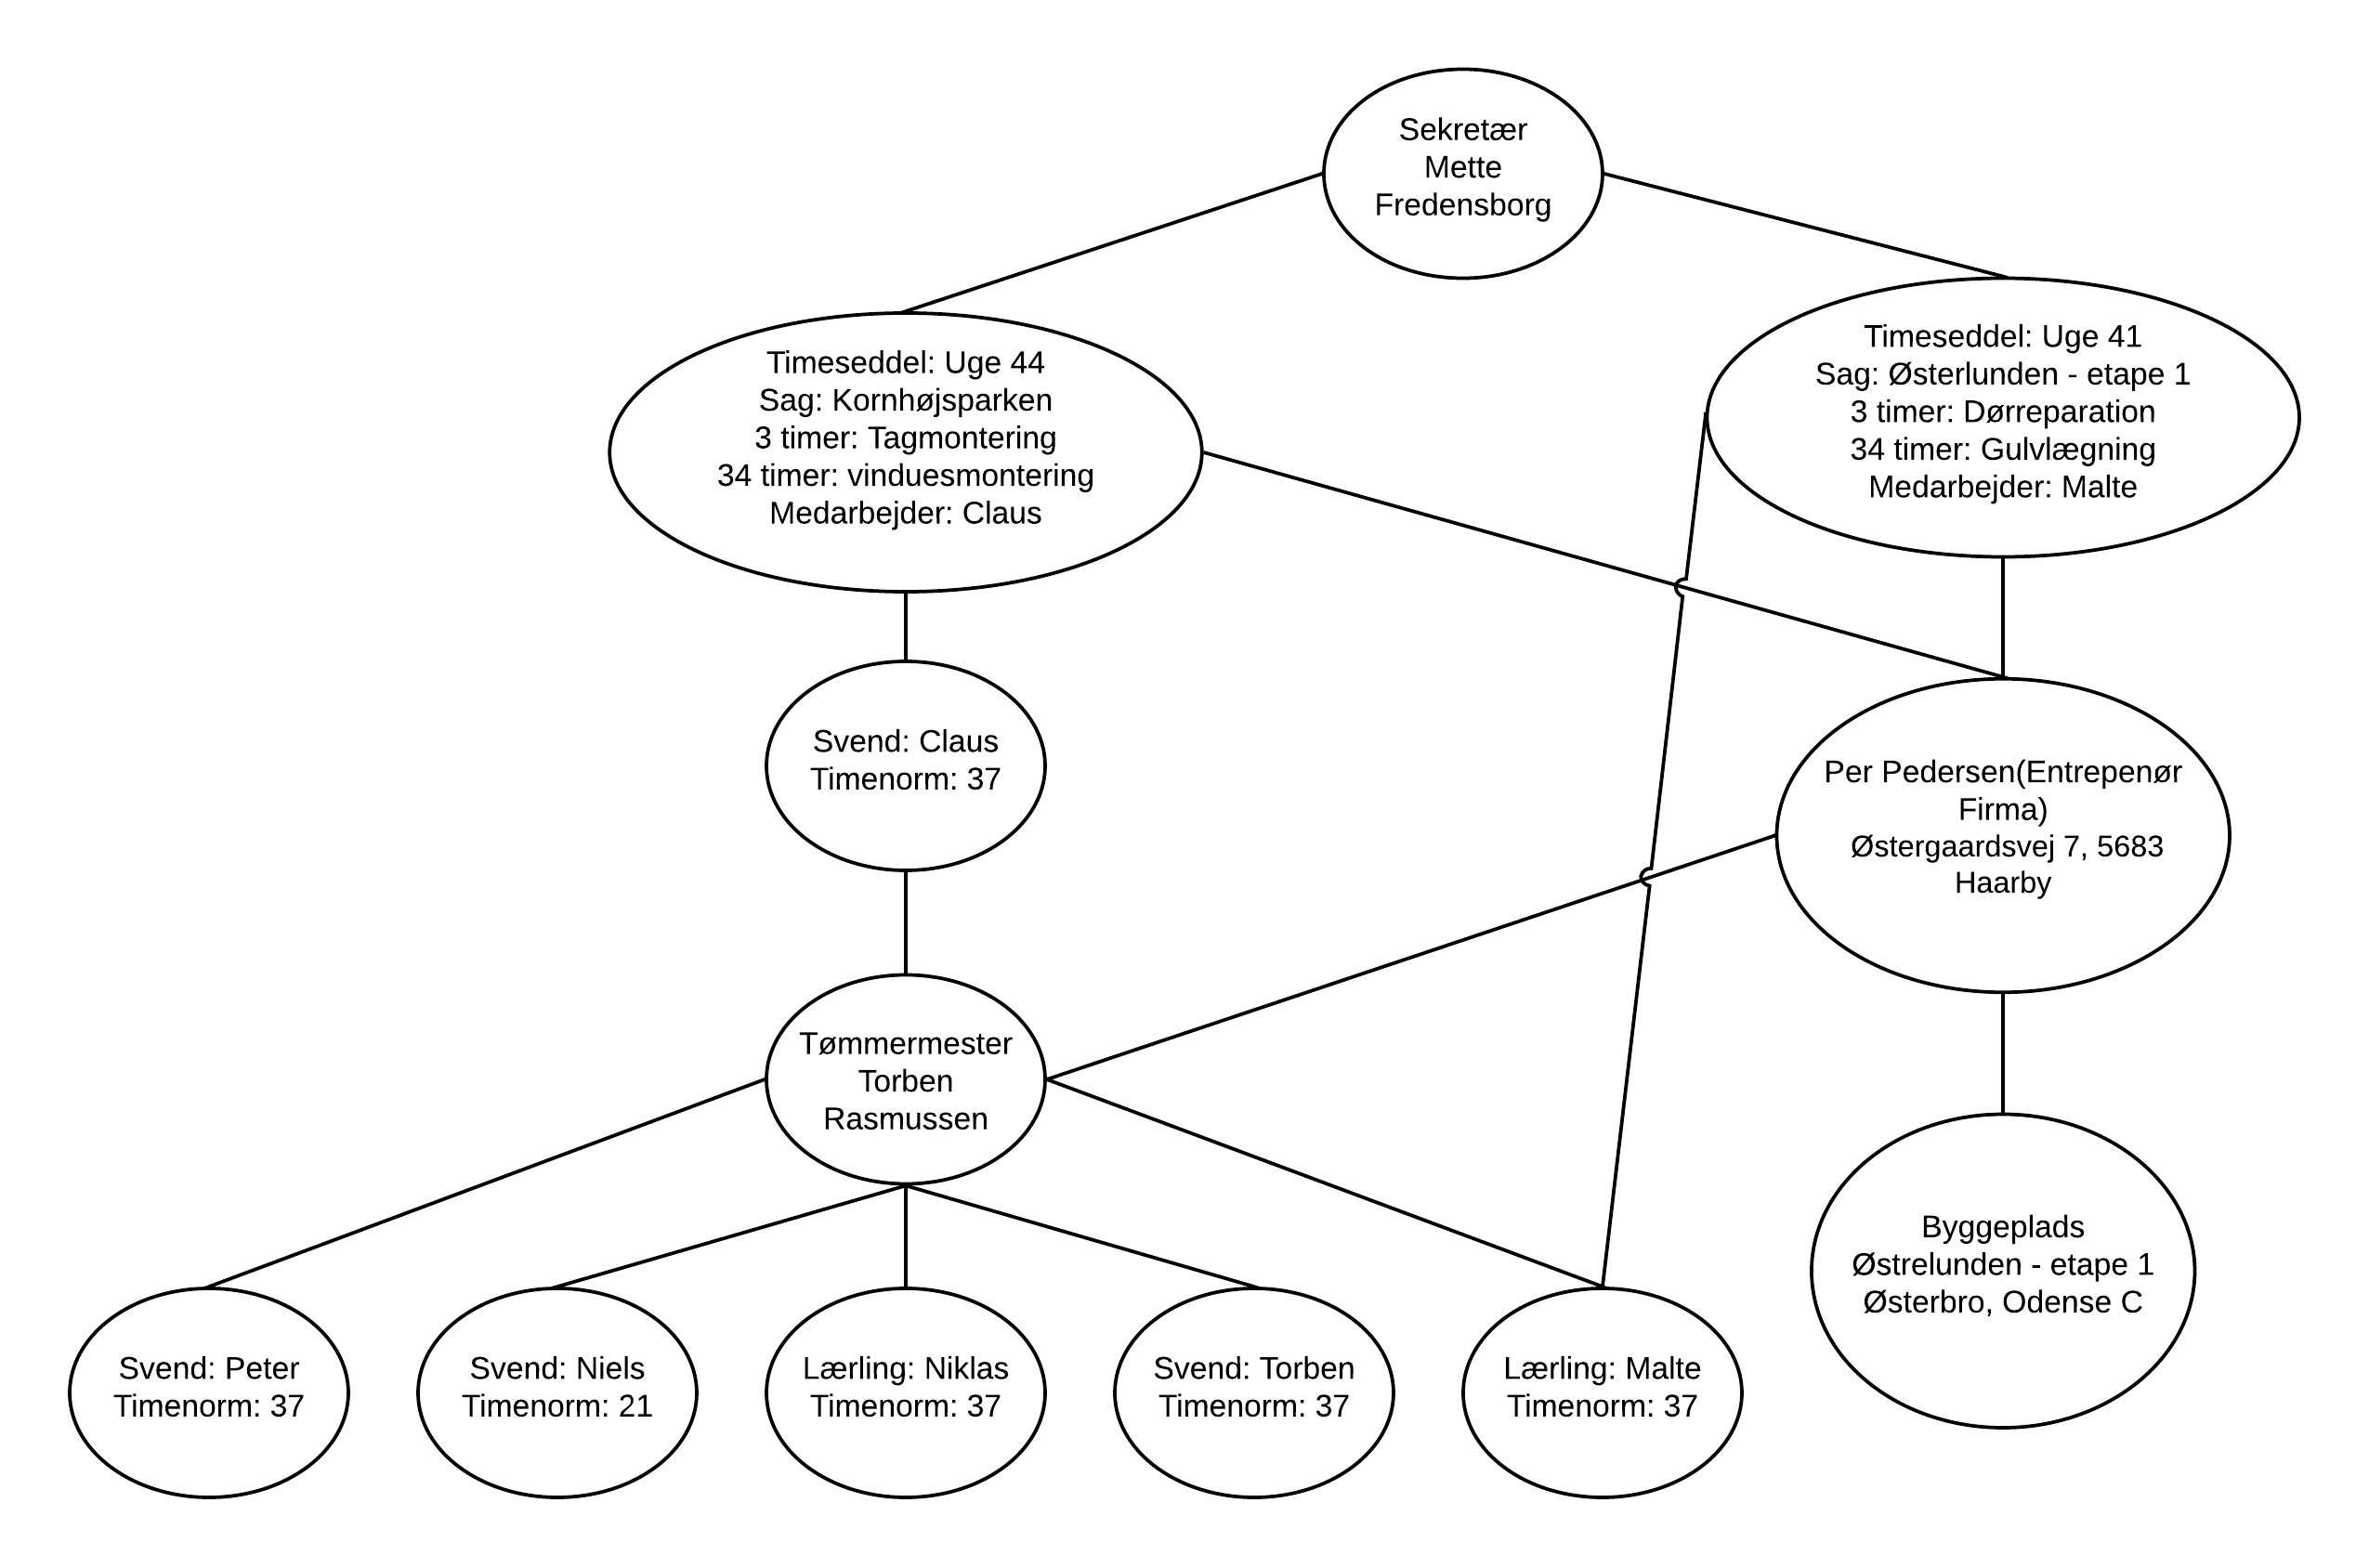
\includegraphics[scale = .6]{ObjektModelSprint2.png}}
    \caption{Objektmodel}
    \label{fig:Objektmodel}
\end{figure}

Der findes flere forskellige objekter. Størstedelen af objekterne er medarbejder objekter. De resterende er timeseddel objekter, byggeplads objekter og kunde objekter. 
\subsection{Domænemodel}

Med en objektmodel opstillet kan vi gå videre og oprette en domænemodel. Domænemodellen har sammen med objektmodellen også gennemgået flere iterationer, hvor klasserne er blevet uddybbet og nogen af dem fjernet. 

Domænemodellen har taget udgangspunkt i at skabe et program for at gøre timeregistrering nemmere. Ud fra vejledningen og erfaringen fra objektmodellen afskaffede vi også værksteds og leverandørs. Ved evt. videreudvikling kunne det være relevant at indfører sådanne klasser, men eftersom de to klasser ikke havde nogen relevans til vores prioriteret PBI blev de undladt.\footnote{Se kapitlet "Fremtidig arbejde" for mere.}
\input{Ordbog}

\begin{comment}
\subsection{Objekt- og Domænemodeller}
\subsubsection{Objektmodellen}
Halvorsen ApS er et firma med mange ansatte, og et strengt hieraki imellem dem.

Det er derfor nødvendigt at differentiere imellem jobstillinger indenfor firmaet.

Udover personalet skal der differentieres mellem forskellige byggepladser.
 
Der er på et givent tidspunkt en til flere byggepladser, og de skal alle sammen registreres til en eller flere sager, og skal så vidt adskilles. 

Det individuelle sager er adskilt med et sagsid. Et eksempel på en sag, ses på objektet "Tagmontering Etape 1". 

I den sag ser man en forbindelse til byggepladsen, hvor tagmonteringen foregår, og yderligere en forbindelse til svenden Torben, som netop er ude og montere tagene. 

Derudover er objekterne sat op med forbindelser, for hvad de har direkte kontakt med.

Her er selvfølgelig udelukket irrelevante faktorer, som fx. at de alle sammen snakker sammen til årets julefrokost. 
\subsubsection Domænemodellen
Ved et første øjekast på domænemodellen, vil man lægge mærke til, at sekretæren kun har ét forhold. Dette forhold defineres ved en én til én forbindelse til tømrermesteren. Som en af de primære brugere af programmet, kan hun derigennem få fuld adgang til resten af firmaet gennem netop tømrermesteren.
\end{comment}
